%%==================================================
%% chapter02.tex for SJTU Master Thesis
%% based on CASthesis
%% modified by wei.jianwen@gmail.com
%% Encoding: UTF-8
%%==================================================

\chapter{流体模拟的基本方法与过完备训练字典技术}
\label{chap:fluidSimulation}

本文研究的内容是一个交叉性课题,主要包括应用重构上采样方法的流体动画计算框架和应用过完备稀疏字典技术的重构上采样方法。在介绍本文研究的流体动画计算框架和过完备稀疏字典方法之前,本章先介绍流体模拟的基本数学模型Navier-Stokes方程组和该模型求解的基本方法,并指出过完备稀疏字典技术重点研究的两个问题。

\section{Navier-Stokes方程组}
\label{sec:navier-stokes}

计算机图形学最有趣的问题之一是类流体行为的仿真,并且,不同的领域,对流体模拟求解的目标要求也有所不同。在特效产业中,模拟流体动画的目的是如何产生令人信服的譬如烟雾、水和火等流体的外观和行为;在计算机动画领域模拟流体动画,我们更关心的则是动画的视觉效果,而不是求解的准确性。尤其对于烟的模拟而言,我们更关心烟动画中的小规模细节,而不是速度场的数值精度。在基于仿真的流体模拟领域,流体力学被作为标准数学框架在使用。科学家们一致表示,Navier-Stokes方程式是模拟流体流动现象的一个很好的数学模型。

\subsection{Navier-Stokes方程组的描述形式}

在流体力学中,Navier-Stokes方程组描述了满足不可压条件的粘性流体,被称为世界上“最复杂的方程之一”。Navier-Stokes方程组的名字记录了推导出该方程组的人的姓名,分别是Claude Louis Navier 和 George Gabriel Stokes,通常也被简称为N-S方程组。可以写成如下形式~\cite{bridson2007fluid}:
\begin{equation}
\label{basicEq}
 \frac{\partial \boldsymbol u}{\partial t} + {\boldsymbol u} \cdot \nabla {\boldsymbol u} + \frac{1}{\rho} \nabla p= {\boldsymbol g} + \nu \nabla \cdot \nabla {\boldsymbol u}
\end{equation}
\begin{equation}
\label{imcompressible}
 \nabla \cdot {\boldsymbol u} = 0
\end{equation}

其中,\(\boldsymbol u\)表示流体的速度场。在欧拉网格方法中,该速度表示流体经过每个固定的点空间时所具有的速度矢量。在3D情况下,\(\boldsymbol u\)通常被写成\((u,v,w)\)的形式,分别表示3D空间标准坐标系下的\(\boldsymbol{x}, \boldsymbol{y}, \boldsymbol{z}\)三个方向上的速度大小。
 
\(p\) 表示压强场,在流体的内部,每个欧拉网格的中心都有存储了一个压强分量。

\(t\)代表时间。
 
\(\nu\)代表流体的粘性系数,\(\nu\)越大,表示流体的粘性越大。
 
\(\rho\)表示流体的密度。
  
 \(\boldsymbol g\)表示施加在流体上的外力合力产生的加速度,这些外力包括重力、浮力等。大部分情况下,流体只受重力的影响,故在此处,我们使用通常表示重力加速度的变量\(\boldsymbol g\)表示流体所受到的外力合力加速度。
 
 \(\nabla\)是向量空间的偏导数, 如\(\nabla {\boldsymbol u}\)表示速度场的偏导数。\(\nabla\) = (\(\frac{\partial}{\partial x}, \frac{\partial}{\partial y})\)表示2D空间的偏导,\(\nabla\) = (\(\frac{\partial}{\partial x}, \frac{\partial}{\partial y}, \frac{\partial}{\partial z})\) 则表示3D空间的偏导。另外,\(\nabla \cdot \nabla\)表示拉普拉斯算子。

\subsection{Navier-Stokes方程组的意义}
\label{sec:eqmeaning}

Navier-Stokes方程组对流体做了以下几个假设:第一,流体是连续的,该假设指液体的内部不能包含空隙,如雾状粒子的聚合、溶解的气泡等。第二,所有涉及到的场都是可微的,如压强场、速度场、密度场和温度场等。

Navier-Stokes方程组的式~\ref{basicEq}根据质量、动量和能量守恒的基本原理导出。我们可以把流体想象成一个粒子系统,每个粒子代表一个小水珠。那么,我们可以描述每个粒子的质量为\(m\),速度为\(\boldsymbol u\),体积为\(V\)。那么根据动量守恒定理,我们可以得到如下方程式:
\begin{equation}
\label{momentum}
 {\boldsymbol F} = m\frac{D{\boldsymbol u}}{D{t}}
\end{equation}

假设粒子受到的来自流体系统以外的力只有重力,表示为\(m{\boldsymbol g}\)。那么我们只需要分析流体粒子来自于粒子系统中其他粒子的力。

\begin{figure}[ht]
  \centering
   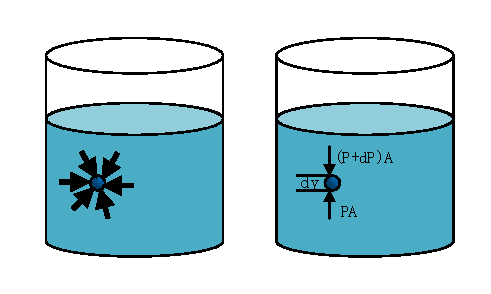
\includegraphics[height=1.8 in]{chap2/pressuredepth}
  \bicaption[pressuredepth]{}{流体粒子受压力示意图}{Fig}{Illustration of how fluid particles are affected by pressure}
\end{figure}

首先是压力。流体在运动的过程中,压力的作用会把高压区的流体推向低压区,从而使得流体粒子在整体上始终保持均匀分布的趋势。图\ref{pressuredepth}画出了流场内部流体粒子受到的所有压力的示意图。从左边的图中,我们可以看出流体粒子所受的压力来自四面八方。我们假设粒子每个方向上所受的压力都相等,根据图\ref{pressuredepth}右边的示例图片,可知流体粒子的压力只与其深度有关。为了简化模型,我们用压强梯度的负值\(-\nabla p\)表示压强的不平衡效果,而\(({-\nabla p})V\)表示粒子所有到的压力。

然后是粘滞力。粘滞力总是阻碍两个粒子之间的相对运动,并且相对运动越大,粘滞力越大。这里,我们直接给出粘滞力的表达式为\(V\mu{\nabla \cdot \nabla {\boldsymbol u}}\)。其中,\(\mu\)为动态粘性系数,是流体自身的属性,通常是常量。故用重力、压力以及粘滞力表示方程式~\ref{momentum}中的外力\(\boldsymbol F\),可得到流体运动的加速度方程:
\begin{equation}
 m\frac{D{\boldsymbol u}}{D{t}} = m{\boldsymbol g} - V{\nabla p} + V{\mu}{\nabla \cdot \nabla {\boldsymbol u}}
\end{equation}

我们已知\(\frac{V}{m} = \frac{1}{\rho}\),设变量\(\nu = \frac{\mu}{\rho}\),上述方程式两边都除以粒子的质量m,则有:
\begin{equation}
 \frac{D{\boldsymbol u}}{D{t}} = {\boldsymbol g} - \frac{1}{\rho}{\nabla p} + {\nu}{\nabla \cdot \nabla {\boldsymbol u}}
\end{equation}

展开速度场\(\boldsymbol u\)关于时间\(t\)的导数,即可得到方程式~\ref{basicEq}。

\begin{figure}[ht]
  \centering
   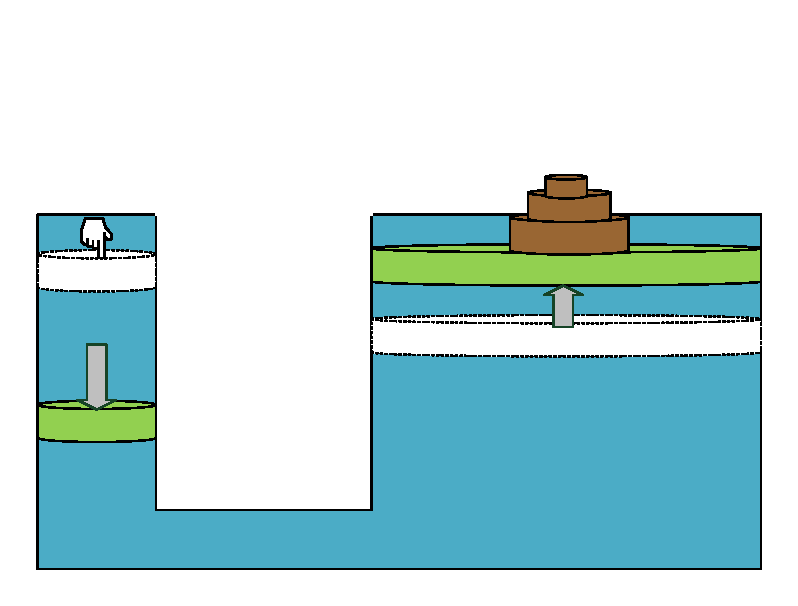
\includegraphics[height=2.3 in]{chap2/imcompressible}
  \bicaption[fig:imcompressible]{}{流体不可压示意图}{Fig}{Illustration of imcompressible condition}
\end{figure}

方程式~\ref{imcompressible}表示流体的不可压缩条件,而图~\ref{fig:imcompressible}展示了流体不可压缩时的宏观表现,即压缩流体时,流体会保持其体积不变。从微观的角度讲,当我们说流体是不可压缩的时,指的是在微观时间段\(\Delta t\)内,流入与流出流体任意体积为\(\Omega\)的流体表面的体积是相等的,即流体的体积变化速率为0,可以表示成如下形式:
\begin{equation}
{\iint_{\partial \Omega}}{\boldsymbol u} \cdot {\hat n} = 0 
\end{equation}

根据微积分基本定理,我们可以将上式转化为如下形式:
\begin{equation}
{\iiint_{\Omega}} \nabla \cdot {\boldsymbol u} = 0 
\end{equation}

由于上述方程式对于流体内部的任意体积\(\Omega\)都是成立的,故只有当被积函数处处为0时,上述函数积分才能为0。当上述积分方程式的被积函数为0时,即可得方程式~\ref{imcompressible}。

\subsection{忽略粘性力作用}

通常,在计算机动画模拟的数值计算中,会忽略掉粘性力这一项。因为相比较于其他作用力,粘性力的值通常是很小的。另外,在流体模拟的数值计算的过程中不可避免地会有数值耗散,而该数值耗散项的值的数量级与粘性力项的值的数量级比较接近,故可以近似认为数值耗散项替代了粘性力项的计算。并且从方程式~\ref{basicEq}中,我们可以看出,粘性力项的计算开销也比较大,忽略粘性力作用可以在很大程度上减少计算的开销。故流体模拟的一般方法求解的是如下形式的Navier-Stokes方程组:
\begin{equation}
\label{basicEqignoreVis}
 \frac{\partial \boldsymbol u}{\partial t} + {\boldsymbol u} \cdot \nabla {\boldsymbol u} + \frac{1}{\rho} \nabla p= {\boldsymbol g}
\end{equation}

\section{流体模拟的基本方法}

根据绪论部分的介绍,可知目前主要的流体模拟方法主要有三大类,即欧拉网格法、拉格朗日粒子法和基于旋度的方法。本文主要研究基于欧拉网格方法的重构上采样框架在流体动画领域的应用,故本章的该部分将会简单介绍用欧拉网格方法求解Navier-Stokes方程组的基本框架。

\subsection{网格介绍}

\begin{figure}
  \centering
   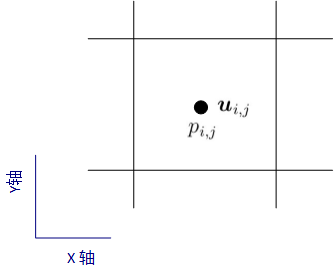
\includegraphics[height=1.6 in]{chap2/centergrid2D}
  \bicaption[fig:centergrid2d]{}{中心网格2D示意图}{Fig}{cells from 2D center grid}
\end{figure}

\begin{figure}[ht]
  \centering
   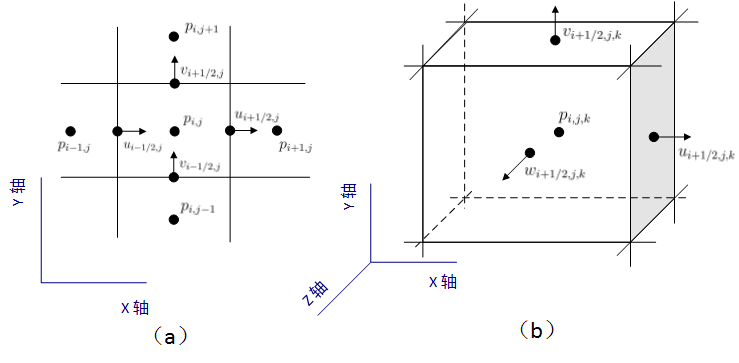
\includegraphics[height=2.5 in]{chap2/macgrid}
  \bicaption[fig:macgrid]{MAC网格示意图}{(a) 2D MAC网格示意图;(b) 3D MAC网格示意图}{Fig}{(a) one cell from the 2D MAC grid;(b) one cell from the 3D MAC grid}
\end{figure}

用欧拉方法求解流体动画时,需要对速度场离散化求解,即在网格上对其进行求解计算。最简单的网格模型是中心网格模型,该网格模型把所有的变量都存储在网格的中心点上,如图~\ref{fig:centergrid2d}描述了中心网格在2D场景下变量的存储方式,其中,$\boldsymbol u_{i,j}$表示位置为$(i,j)$处的网格点的速度场矢量,$p_{i,j}$表示同一网格位置的压强场。但是被更为广泛使用的是MAC网格模型,由Harlow等人~\cite{harlow1965numerical}提出。MAC网格实际上是一个交错的网格,变量存储在网格的不同位置上,并且存储在不同位置的变量有不同的含义,如图~\ref{fig:macgrid}所示,(a)和(b)分别描述了2D场景和3D场景下MAC网格各变量的存储方式,其中\(p\)是压力值,\(u,v,w\)分别表示速度场的三个分量。相较于中心网格,MAC网格的计算效率更高,并且更加稳定,故在欧拉网格方法中使用更为广泛。本文提出的流体模拟重构框架既适用于中心网格,也适用于MAC网格。

\subsection{欧拉网格方法及其计算框架}

Navier-Stokes方程组方程组虽然看起来简单,但是因为方程式~\ref{basicEqignoreVis}存在非线性项,故直接求解非常困难。为了简化求解过程,通常会把Navier-Stokes方程组分解成三个部分求解,分别为对流、体积力和压力/不可压缩部分。分别列出如下:
\begin{equation}
\label{eq:advection}
\frac{\partial {\boldsymbol u}}{\partial t} + {\boldsymbol u} \cdot \nabla {\boldsymbol u} = 0  \ \ \ \ \ (advection)
\end{equation}
\begin{equation}
\label{eq:addForce}
\frac{\partial {\boldsymbol u}}{\partial t} = {\boldsymbol g}  \ \ \ \ \ \ (body forces)
\end{equation}
\begin{equation}
\label{eq:projection}
\frac{\partial {\boldsymbol u}}{\partial t} + \frac{1}{\rho} \nabla p= 0 
\ \ \ \ \ 
 s.t. \ \ \ \ \ 
 \nabla \cdot {\boldsymbol u} = 0 \ \ \ \ \ \ (pressure/incompressibility)
\end{equation}

上述三个方程式通常对应欧拉方法的三个步骤,即式~\ref{eq:advection}对应对流步,通常表示为advection,该步骤把速度场\({\boldsymbol u}\)对流一个时间间隔\(\Delta t\);式~\ref{eq:addForce}对应外力步,表示成addForce,表示外力合力作用对流体速度场的加速度;式~\ref{eq:projection}对应投影步,表示为projection,该步骤保证前两步计算得出的速度场\({\boldsymbol u}\)是无散的,同时还保证流体速度场满足固体边界条件。

在这三个部分中,我们需要保证对流是在无散速度场中进行的,故advection步骤的运行需要以projection步骤的输出为前提。综上所述,可以归纳出欧拉网格方法的基本运算步骤如算法~\ref{Eulerframework}所示。

\begin{algorithm}%[htb]
\caption{ 流体模拟的基本框架伪代码.}
\label{Eulerframework}
\begin{algorithmic}[1] %这个1 表示每一行都显示数字
%\REQUIRE ~~\\ %算法的输入参数:Input
%coupled dictionaried $\boldsymbol D_l \ and \ \boldsymbol D_h$, low-resolution fluid velocity field $\bar {\boldsymbol u}$.
%\ENSURE ~~\\ %算法的输出:Output
%high-resolution fluid velocity field $\boldsymbol U$. 
  \STATE initialize a divergence-free velocity field ${\boldsymbol u}^{(0)}$;
\FOR{ every time step  $n = 0, 1, 2, ...$} 
    \STATE Do the advection: ${\boldsymbol u}^{A} = advection({\boldsymbol u}^n, \Delta t)$.
    \STATE  Do the addForce: ${\boldsymbol u}^{B} = {\boldsymbol u}^{A} + {\Delta t} {\boldsymbol g}$. 
    \STATE Do the projection: ${\boldsymbol u}^{n + 1} = projection({\Delta t}, {\boldsymbol u}^{B})$.
\ENDFOR
\end{algorithmic}
\end{algorithm}

根据Navier-Stokes方程组的三个分解方程式,可以看出流体模拟的三个步骤中,最为耗时的是投影步骤。该步骤实际上求解的是一个泊松方程,Stam~\cite{stam2003real}使用了经典的高斯赛德尔迭代方法求解,Foster 等人~\cite{foster2001practical}采用了预处理共轭梯度法(ICPCG)求解,ICPCG 因其优秀的性能,成为了求解投影步骤的主流。但是投影步骤仍然是流体模拟方法的瓶颈步骤。

在Stam~\cite{stam1999stable}提出了允许大时间步长的无条件稳定的半拉格朗日方法求解对流步骤之后,很多人针对如何提高对流步骤数值解的精度提出了一些改进方案,如MacCormack~\cite{selle2008unconditionally},BFECC~\cite{kim2005flowfixer}~\cite{dupont2003back},QUICK~\cite{molemaker2008low}等对流方法。这些对流方法在一定程度上丰富了流体动画的细节,并且相较于投影步骤,其计算开销可以忽略不计。

\section{基于稀疏编码的过完备稀疏字典技术}

近几年来,研究使用稀疏编码技术获取信号的稀疏表示形式成为了一个热门话题,并应用到图像去噪~\cite{donoho1995noising}、图像修复、图像超分辨~\cite{yang2008image}等许多图像处理领域。过完备的稀疏字典包含信号的特征基原子,可以通过字典中的很少一些原子的线性组合表示原信号~\cite{aharon2006overcomplete}。通常来讲,基于稀疏编码技术的稀疏字典方法主要集中于求解两个问题:(1)训练合成过完备稀疏字典的方法;(2)执行稀疏分解及性能分析的算法。

\subsection{训练过完备稀疏字典}

字典学习的方法可以描述成如下问题~\cite{aharon2006overcomplete}:给定一个信号的集合$\{\boldsymbol x_i\}_{i = 1}^{N}$,这些信号的集合可以根据一个未知的字典$\boldsymbol D$获取其稀疏表示形式,我们要如何才能找到这个未知的字典$\boldsymbol D$?通常,字典$\boldsymbol D$必须是唯一的,并且能够尽可能逼近地表示所有给定信号$\{\boldsymbol x_i\}_{i = 1}^{N}$。

设${\boldsymbol D} \in {\boldsymbol R}^{k \times n}$是具有$k$个原型信号基原子的过完备字典,信号$\boldsymbol x \in \boldsymbol R^{n \times 1}$可以由字典中原子的稀疏线性组合表示,表示成$\boldsymbol x = \boldsymbol {D\alpha}$,或者近似表示成$\boldsymbol x \approx \boldsymbol {D\alpha}$,其中,向量$\boldsymbol \alpha$是信号的稀疏表示系数。当我们称向量$\boldsymbol \alpha$是信号的稀疏表示时,指向量$\boldsymbol \alpha$中只有很少的非零元素。通常使用$l^p$范数求解上述近似问题,$p = 1,2$或者 $\infty$。在构造稀疏字典的方法中,通常取$p = 2$,故训练过完备稀疏字典的方法可以表示成如下方程式:
\begin{equation}
\label{eq:sparseRep}
\min_{\boldsymbol  \alpha}||\boldsymbol \alpha||_0 \ \ \ s.t. \ \ \ ||\boldsymbol x - \boldsymbol {D\alpha}||_2 \leq \epsilon
\end{equation}

提取信号的最稀疏表示是一个NP-hard问题。近几年的研究中,出现了一些较为高效的近似分解算法,如K-SVD~\cite{aharon2006svd}算法、标记特征搜索(Feature-sign search)~\cite{lee2006efficient}算法等。这些算法在求解的过程中,都需要假定待求的稀疏字典是已知并且固定的,然后再通过迭代的方式计算出最优解。

目前,学习过完备稀疏字典的学习方法主要集中于在一个单一特征空间内为各种恢复、识别的任务训练过完备稀疏字典。然而,在很多应用和实际场景中,却有两个特征空间,如超分辨技术中的高精度和低精度信号空间。学习这样的一对低—高精度稀疏字典,无论是在信号处理还是在计算机视觉中,都有很多应用,比如压缩感知~\cite{donoho2006compressed}等。Yang~\cite{yang2012coupled}等人提出了学习低清晰度和高清晰度图像patch的联合字典学习方法,这个方法将两个特征空间联接起来,然后将其转化为标准的单特征空间稀疏编码问题,故也可以通过上述提到的近似算法求解。本文中,我们希望重构上采样低精度网格速度场数据到高精度速度场空间,因此也需要学习一对稀疏字典。

\subsection{信号的稀疏分解问题}

设${\boldsymbol D} \in {\boldsymbol R}^{n \times k}$是具有$k$个原型信号基原子的过完备字典,并假设信号\({\boldsymbol x}  \in {\boldsymbol R}^{n \times 1}\) 可以表示为一个这些元素的稀疏线性组合,也就是说,信号集合\({\boldsymbol x}\)可以写成${\boldsymbol x} = {\boldsymbol D} \boldsymbol \alpha_0$的形式,其中$\boldsymbol \alpha_0 \in  {\boldsymbol R}^{k \times 1}$是稀疏表示系数。在图像超分辨环境下,我们可能只知道一小组由${\boldsymbol x}$表示的测量值${\boldsymbol y \in \boldsymbol R^{m \times 1}}$组成的集合:
\begin{equation}
\label{eq:linear}
\boldsymbol y = \boldsymbol L \boldsymbol x =\boldsymbol L \boldsymbol {D\alpha}_0
\end{equation}

其中,$\boldsymbol L \in {\boldsymbol R}^{m \times n}, m < n$ ,$\boldsymbol L$代表降采样等操作,$\boldsymbol x$表示高精度信号原子,而$\boldsymbol y$是它的低精度版本。信号的稀疏分解问题求解的问题是,给定低精度信号$\boldsymbol y$,根据过完备稀疏字典$ {\boldsymbol D}$求解出低精度信号$\boldsymbol y$的稀疏表示形式$\boldsymbol \alpha_0$。用公式的形式表示信号的稀疏分解问题,可写成如下形式:

\begin{equation}
\min_{\boldsymbol  \alpha_0}||\boldsymbol \alpha||_0 \ \ \ s.t. \ \ \ ||\boldsymbol y - \boldsymbol {LD\alpha}_0||_2 \leq \epsilon
\end{equation}

上述公式也是一个NP-hard问题,故无法精确分解出低精度信号$\boldsymbol y$的稀疏表示形式$\boldsymbol \alpha_0$。但是,针对上述公式,目前已经提出了很多的近似解法,如追踪匹配(Matching pursuit)~\cite{mallat1993matching}、基追踪~\cite{chen1998atomic}、FOCUSS~\cite{rao1997deriving}以及由这些算法衍生出的其他近似算法等。追踪匹配算法的核心思想是使用贪婪算法顺序地选取最优的字典基原子,这类算法比较简单;基追踪算法通过将稀疏系数$\boldsymbol \alpha$的$l^0$范数约束条件转换成$l^1$范数的最凸解问题对原信号做分解计算;FOCUSS算法与基追踪算法的思想十分类似,但不同的是,FOCUSS算法使用$l^p$范数约束替换原公式的$l^0$范数约束,其中$p \leq 1$。

本文应用基于稀疏编码技术的稀疏字典方法也主要集中于求解上述两个问题,第四章将会详细介绍本文的解决方案。

\section{本章小结}

本章介绍了流体动画技术的数学模型Navier-Stokes方程组,并且详细地给出了方程组的推导过程以及每个部分的具体含义。同时,本章还介绍了欧拉方法常用的网格模型,以及欧拉方法的基本框架。流体模拟的一般方法将流体的数值计算分成了三个步骤,对流、加外力和投影步骤,其中,对流和加外力步骤相较于投影步骤,其时间开销可以忽略不计。为了解决在提高求解网格的精度时,投影步骤的计算过于昂贵这一问题,引入了本文在第三章节将要提出的应用过完备稀疏字典技术的流体模拟重构上采样框架,将高耗时的投影步骤放到低精度网格上去计算,从而达到减少投影步骤时间耗费的目的。

本章还简单地介绍了基于稀疏编码的过完备字典技术,以及该技术主要集中求解的两个问题,即稀疏字典的学习方法和信号的分解算法。学习一对过完备稀疏字典,是本文的一个重点内容。在本文的第四个章节将会详细地介绍Yang提出的联合双字典方法,以及本文对该重构方法的改进,达到提高重构结果准确性的目的。